\documentclass[journal]{IEEEtran}

\hyphenation{op-tical net-works semi-conduc-tor}

\usepackage{amsmath}
\usepackage{amssymb}
\usepackage{amsthm}
\usepackage{graphicx}
%\usepackage{hyperref}

\newtheorem{mydef}{Definition}
\newtheorem{mylem}{Lemma}
\newtheorem{mythm}{Theorem}
\newtheorem{myprop}{Property}
\newtheorem{mycoro}{Corollary}


\begin{document}

\title{Understanding the Particle Swarm Optimization by component decomposition}

\author{
\IEEEauthorblockN{Daqing Yi,
Kevin D. Seppi, and Michael A. Goodrich}

\IEEEauthorblockA{Department of computer science, Brigham Young University, Provo, UT 84604 USA}
\thanks{}
}

% The paper headers
%\markboth{Journal of \LaTeX\ Class Files,~Vol.~11, No.~4, December~2012}%
%{Shell \MakeLowercase{\textit{et al.}}: Bare Demo of IEEEtran.cls for Journals}
\markboth{}{}

\maketitle

\begin{abstract}
The stochastic behaviors of the particles and the swarm structure empower the capability of optimal search in PSO.
As well they increase the difficulty of understanding the dynamics of the PSO, i.e., whether the PSO will converge and how the PSO will converge.
The common methods of analyzing the PSO reply on the simplification of the algorithm, e.g., using stagnation assumption (a state where the swarm ceases finding better solutions) and constantizing the stochastic factors.
In this paper, we analyze the dynamics of the PSO by decompose the swarm and the particles into components.
We import input-to-state stability analysis to the decomposed components, which allows us to know the behavior of the convergence from a single particle to the entire swarm.
It enables the analysis of the PSO without any simplification and includes the influence to the particle when running in a swarm structure.


%Previous analysis of the dynamics of particle swarm optimization has often relied on either the assumption of ``stagnation'' (a state where the swarm ceases make progress), the removal of random effects, or both.
%In this paper we use a newer tool for the analysis of system dynamics, specifically the concept of Input to State Stability (ISS).
%ISS allows us to make statements about the behavior of the swarm not clearly address in previous analysis, specifically bounds on particle and swam behavior.
%We can also do so before stagnation and with random affect fully accounted for. 
\end{abstract}

\begin{IEEEkeywords}
Particle swarm optimization
\end{IEEEkeywords}

\IEEEpeerreviewmaketitle

\section{Introduction}
\label{sec:intro}

This project is based on ``Distributed cooperative attitude synchronization and tracking for multiple rigid bodies'' by Dr. Ren \cite{5229134}, in which discusses the consensus seeking of a system of agents with non-linear model.
Two approaches have been proposed for ``cooperative attitude synchronization'' (position control) and ``reference attitude tracking'' (trajectory tracking) respectively.
Two approaches are stated independently and look different.
One objective of this project is seeking the consensus between two approaches, which can be used as a pattern on analyzing other synchronization systems and designing control laws for them.

The structure of this report is as following.
Section \ref{sec:prob_stat} states the system model, which includes the rigid body dynamics of each agent and the interaction topology.
Section \ref{sec:coop_att_syn} presents the control law proposed for the cooperative attitude synchronization and the proof strategy.
%I try to figure out the roles of the terms in the control law so that I can simplify the control law with ignorance on the transient performance and prove the stability.
By analyzing the roles of the terms in the control law, I simplify the control law to find the essential component that guarantees the stability.
It means that the stability can still be preserved and proved without some terms for transient performance.
Section \ref{sec:ref_att_trk} illustrates the control law proposed for the reference attitude tracking and the proof strategy.
I use a same proof strategy to prove the stability of the control law on the cooperative attitude synchronization, which shows the consistency between two approaches.
It means that the ideas of improvement can be applied to both control approaches.
Simulations are also taken on both approaches for analysis purpose.
Section \ref{sec:io_stable} proposes an interconnection perspective for analyzing a class of distributed system control problems as a pattern of analyzing a consensus-seeking problem.
A hypothesis on proving the stability is proposed, in which the proof can be achieved by analyzing the stability-relevant properties of the sub-components.
Section \ref{sec:summary} discusses some possible future work from Dr. Ren's paper.

\section{Related work}
\label{sec:rel_work}

Although the input-to-state stable analysis given in this paper can be applied to many versions of PSO,
for this work we use the formulas from Kennedy's most recent definition of PSO\cite{4223164}.
This version of PSO includes a ring topology, and a constricted position update rule. 
The constricted position update rule is

\begin{subequations}
\label{eq:pso_alg}
\begin{equation}
\label{eq:up_vel}
\begin{aligned}
v_{ij}(k+1) & = \chi [ v_{ij}(k) 
 + \phi^{P} u^{P}_{ij}(k) (x^{P}_{ij}(k) - x_{ij}(k)) + \phi^{G} u^{G}_{ij}(k) ( x^{G}_{ij}(k) - x_{ij}(k)) ],
\end{aligned}
\end{equation}
\begin{equation}
\label{eq:up_pos}
x_{ij}(k+1) = x_{ij}(k) + v_{ij}(k+1).
\end{equation}
\end{subequations}
$ x_{ij}(k) $ represents the position of particle $ i $ in dimension $ j $ at time $ k $.
$ v_{ij}(k) $ similarly represents the velocity of particle $ i $ in dimension $ j $ also at time $ k $.
$ x^{G}_{ij}(k) $ and $ x^{P}_{ij}(k) $ are global (actually topology) and personal best positions observed by the swarm and the particle respectively. 
$ u^{G}_{ij}(k) $ and $ u^{P}_{ij}(k) $ are independent random values drawn from $ [0,1] $.
$ \chi \in ( 0, 1 ) $, $ \phi^{P} $ and $ \phi^{G} $ are algorithm parameters.

Due to the stochastic nature of the particle's path and the social interaction represented by the topology, the dynamics of the algorithm is hard to evaluate in general.
However once a particle is no longer able to find improvements in $ x^{G} $ and $ x^{P} $, it exhibits the \emph{stagnation phenomenon} \cite{Clerc06stagnationanalysis}.
In this state the analysis is easier since there is no effect from the topology.

Previous work that assumes stagnation can be categorized into two groups each based on how the analysis treats the stochastic factors.
The first approach is to ignore the stochastic factors.
Using this simplification, the convergence of a particle at stagnation can be analyzed \cite{985692}. 
By building a linear system model \cite{4424687}, the PSO algorithm can be viewed as a closed loop system and the convergence can be analyzed.
Based on such a convergence analysis, parameters can be set for best effect \cite{Trelea2003317}.

The second approach for handling the stochastic factors is based on the stochastic analysis.
By taking the mean of the stochastic variables, the stochastic terms can be converted into
constant terms.
A convergence analysis of the mean and variance of a particle at stagnation can also be obtained using the characteristic equation in a discrete-time model 
\cite{Jiang20078}.
In a similar way, 
other moments can be computed
\cite{5175367,Poli:2007:EAS:1276958.1276977,Poli:2008:DSS:1384929.1384944}.
Using the discrete-time system model of different moments, the equilibrium can be found.
The stability requirements can be obtained from the norm by setting the root values of the characteristic equation to all be less than 1.

There is also some work that addresses the dynamics when a particle is not in the stagnation phase.
The discrete-time dynamics of PSO, that is, the dynamics of particle trajectory, can be approximated
using a continuous-time model
\cite{5675669}.
Furthermore, the probability of convergence in time can be analyzed
by viewing the update process as a random search process
\cite{vandenBergh:2010:CPP:2010420.2010421}.
The process of particles reaching a local optimum
has also been analyzed
\cite{Schmitt:2013:PSO:2463372.2463563}.

\section{System}
\label{sec:system}

When the position of a particle is chosen to be the global best, its personal best is updated as well.
In this case, $ x(k) = x^{P}(k) = x^{G}(k) $, which means this particle will not move till a new global best is found.
We could view this particle as a leader of this swarm.
The topology is given in Figure \ref{fig:leader_follower}.

\begin{figure}[tbph]
\centering
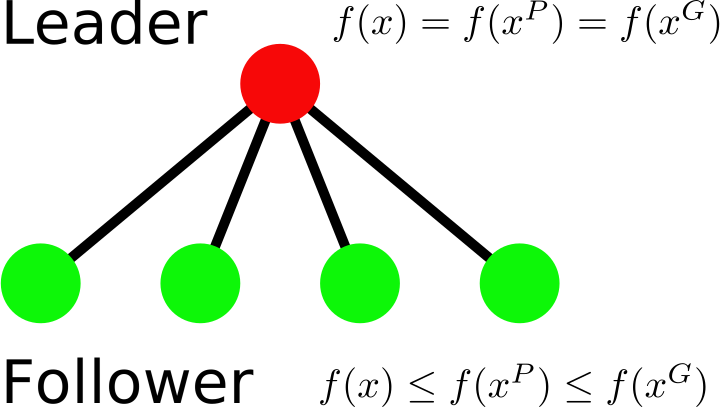
\includegraphics[width=0.5\linewidth]{./fig/leader_follower}
\caption{}
\label{fig:leader_follower}
\end{figure}


The optimal search process of the swarm becomes a leader competition among the particles.
Once a particle finds a new global best, it becomes the leader of the swarm.
The other particles are the followers, which are attracted to the leader by the impact of the global best.
By Property \ref{prop:unconverge_neq_gb}, we know that a particle will never stop moving if the personal best and the global best are inconsistent.
Thus, we can view the movements of the followers are sampling in the solution space to solve the inconsistency between its own personal best and the global best.






\section{Input-to-state stability}
\label{sec:iss}

%\begin{itemize}
%\item ISS of a particle (use an appendix if long)
%\item Parameters need for a particle to be ISS
%\item Contrast with the empirical approach of Clerc and Kennedy??
%\item Use appendix for mean and variance analysis
%\end{itemize}

The properties of this system can be analyzed using the input-to-state stability of the position update component. 
Given an input-to-state stable position update component, we will see that the convergence of $ x_{i}(k) $ depends on bounds on $ x^{G}_{i}(k) $ and $ x^{P}_{i}(k) $.

Without loss of generality, we look at a one-dimension particle.
The parallel connection of input-to-state stable components reserves the input-to-state stability.

In our analysis of the PSO algorithm, we seek to understand how the particles converge to some position $ x^{*} $, which is intended (not guaranteed) by the algorithm to be the optimal position.
The convergence of this model means that $ v(k) \rightarrow 0 $ and $ x(k) \rightarrow x^{*} $.

\subsection{Input-to-state stability of the position update}

In this section, we briefly review the definition of input-to-state stability (ISS) including both the conditions that guarantee it and the bound that ISS implies\cite{Jiang2001857}. 
We then show that PSO satisfies this definition when the parameters of PSO are set in the requisite range.
We also derive the bounds implied by the ISS property.
We use the ISS property to find bounds on particle motion.

We first introduce several types of functions \cite{Jiang2001857}.
\begin{itemize}
\item $ K $-function $ \mathbb{K} $ : a function $ \alpha  : [ 0, a ) \rightarrow [ 0, \infty ) $ is continuous, strictly increasing and $ \alpha (0) = 0 $; it is a $ K_{\infty} $-function, if $ \alpha (s) \rightarrow \infty $ as $ s \rightarrow \infty $;
\item $ KL $-function $ \mathbb{KL} $ : a function $ \beta : [ 0, a ) \times [ 0 , \infty ) \rightarrow [ 0, \infty ) $ satisfies:
\begin{enumerate}
\item $ \forall t \geq 0 $, $ \beta (\cdot , t ) $ is a $ K $-function;
\item $ \forall s \geq 0 $, $ \beta (s, \cdot) $ is decreasing and $ \beta(s,t) \rightarrow 0 $ as $ t \rightarrow \infty $.
\end{enumerate}
%\item Positive-definite function: a function $ \gamma (s) > 0, \forall s > 0 $ and $ \gamma (0) = 0 $.
\item ISS-Lyapunov function $ V : \mathbb{R}^{n} \rightarrow \mathbb{R}_{\geq 0} $ satisfies:
\begin{enumerate}
\item $ \exists \alpha_{1}, \alpha_{2} \in \mathbb{K} $ such that 
$ \forall \xi \in \mathbb{R}^{n}, \alpha_{1} ( | \xi | ) \leq V( \xi ) \leq \alpha_{2}  ( | \xi | ) $.
\item $ \exists \alpha_{3} \in \mathbb{K}_{\infty} , \sigma \in \mathbb{K} $ such that $ \forall \xi \in \mathbb{R}^{n}, \forall \mu \in \mathbb{R}^{m}, V( f( \xi, \mu ) ) - V( \xi ) \leq - \alpha_{3} ( | \xi | ) + \sigma ( | \mu | ) $. 
\end{enumerate}
\end{itemize}

\begin{mydef}[Input-to-state stable]\cite{Jiang2001857}
\label{def:iss}
For a discrete-time system
\begin{equation}
\label{eq:dis_nonlinear}
x(k+1) = f( x(k) , u(k) ),
\end{equation}
with $ f(0,0) = 0 $
\footnote{This means that $ x = 0 $ is an equilibrium of the 0-input system.}, the system is \emph{(globally) input-to-state stable} if there exist a $ KL $-function $ \beta  $ and a $ K $-function $ \gamma $ such that, for each input $ u \in l^{m}_{\infty} $ and each $ \xi \in \mathbb{R}^{n} $, it holds that $  \forall k \in \mathbb{Z}^{+} $,
\begin{equation}
\label{eq:def_iss}
| x(k, \xi, u) | \leq \beta (| \xi |, k) + \gamma ( \lVert u \rVert ).
\end{equation}
\end{mydef}

The $ \beta () $ term in \eqref{eq:def_iss} defines an initial bound with a decaying property.
The $ \gamma () $ term in \eqref{eq:def_iss} defines a bound determined by the input.
This means that the influence $ \beta () $ term gradually decreases to zero and the position is bounded by a range determined by the bound on the input.
An ISS-Lyapunov function, defined above, can be used to prove the input-to-state stability of a system and analyze the state bound\cite{Jiang2001857}.
We will use the ISS-Lyapunov-function approach in the proof given later in this section.

\subsection{Conditions for input-to-state stability for position update in PSO}

Using the definition of the PSO position update as given in \eqref{eq:pso_up_linalg_simp}, PSO can be shown to be ISS as defined in definition \ref{def:iss}.

\begin{mythm}
\label{thm:iss}
The system \eqref{eq:pso_up_linalg_simp} is input-to-state stable, when $ | \lambda_{\max} ( A(k) ) | < 1 $.
%The system \eqref{eq:pso_up_linalg_simp} is input-to-state stable, if there exists a symmetric positive definite matrix $ P $ and a symmetric positive definite matrix $ Q' $ that has $ A(k)^{T} P A(k) - P = - Q(k) \leq - Q' $.
\begin{proof}

Let $ P $ be an identity matrix.
As $ | \lambda_{\max} ( A(k) ) | < 1 $, we have
$ \lVert A^{T}(k) P A(k) \rVert \leq \lVert P \rVert \lVert A(k) \rVert^{2} \leq \lVert P \rVert | \lambda_{\max} ( A(k) ) |^{2} < \lVert P \rVert $.
Because $ P $ is an identity matrix it is positive definite, and thus $ A^{T}(k) P A(k) $ is positive definite or positive semi-definite by definition.
So by positive definite ordering we have $ A^{T}(k) P A(k) < P $.

Let $ -Q(k) = A^{T}(k) P A(k) - P $. Since $ A^{T}(k) P A(k) < P $ then $ - Q(k) < 0 $ furthermore $ \exists Q' \forall k, Q(k) > Q' > 0 $. 

By the Lemma 3.5 in \cite{Jiang2001857}, if we can show that a proposed positive definite Lyapunov function is an ISS-Lyapunov function, then the system is ISS.

Define a Lyapunov function
\begin{equation}
\label{eq:lyapunov_v}
V( X(k) ) = X^{T} (k) P X(k).
\end{equation}
We can have
$
\lambda_{min}(P) | X(k) |^{2} \leq V( X(k) )\leq \lambda_{max}(P) | X(k) |^{2}
$ and $ \lambda_{min}(P) = \lambda_{max}(P) $.

Let $ \alpha_{1} ( \xi )= \lambda_{min} \xi^{2} $
and 
$ \alpha_{2} ( \xi )= \lambda_{max} \xi^{2} $,
we have $ V(x) $ satisfying condition 1 of the ISS-Lyapunov function definition.

By applying \eqref{eq:pso_up_linalg_simp} to $ V( X(k+1) ) - V( X(k) ) $, we have
\begin{equation}
\label{eq:lyapunov_delta2}
\begin{aligned}
& V( X(k+1) ) - V( X(k) ) \\
= & - X^{T}(k) [ A^{T}(k) P A(k) - P ] X(k)  \\
& + 2 X^{T}(k)  A^{T}(k) P B(k) U(k) + U^{T}(k) B^{T}(k) P B(k) U(k) \\
\leq & - X^{T}(k) Q' X(k) + 2 X^{T}(k)  A^{T}(k) P B(k) U(k) \\
& + U^{T}(k) B^{T}(k) P B(k) U(k) \\
\leq & - \lambda_{min}(Q') | X(k) |^{2} + 2  \lVert A^{T}(k) P B(k) \rVert | U(k) | | X(k) | \\
& + \lVert B^{T}(k) P B(k) \rVert | U(k) |^{2}.
\end{aligned}
\end{equation}

By completing the square, we have
\begin{equation}
\label{eq:lyapunov_delta4}
\begin{aligned}
& V( X(k+1) ) - V( X(k) ) \\
\leq & - \frac{1}{2} \lambda_{min}(Q') | X(k) |^{2} + [ \frac{2 \lVert A^{T}(k) P B(k) \rVert^{2}}{ ( \lambda_{min}(Q') )^{2} }  \\
& + \lVert B^{T}(k) P B(k) \rVert ] | U(k) |^{2}. 
\end{aligned}
\end{equation}

Because $ u^{P}(k) \in [0, 1] $, there exist an $ A' $ and $ B' $ such that $ \lVert A(k) \rVert \leq \lVert A' \rVert $ and $ \lVert B(k) \rVert \leq \lVert B' \rVert $.
We have $ \lVert A^{T}(k) P B(k) \rVert \leq \lVert A' \rVert \lVert P \rVert \lVert B' \rVert $ and $ \lVert B^{T}(k) P B(k) \rVert \leq \lVert P \rVert \lVert B' \rVert^{2} $.

Since the identity matrix $ P $ has $ || P || = 1 $:
\begin{equation}
\label{eq:lyapunov_delta5}
\begin{aligned}
& V( X(k+1) ) - V( X(k) ) \\
\leq & - \frac{1}{2} \lambda_{min}(Q') | X(k) |^{2} + [ \frac{2 \lVert A' \rVert^{2} \lVert B' \rVert^{2}}{ ( \lambda_{min}(Q') )^{2} } + \lVert B' \rVert^{2} ] \lVert U(k) \rVert^{2}.
\end{aligned}
\end{equation}

Let
$ \alpha_{3} ( \xi )= \frac{1}{2} \lambda_{min}(Q') \xi^{2} $,
and
$ \sigma ( \xi ) = [ \frac{2 \lVert A' \rVert^{2} \lVert B' \rVert^{2}}{ ( \lambda_{min}(Q') )^{2} } +  \lVert B' \rVert^{2} ] \xi^{2} $.
Thus we have $  V( X(k+1) ) - V( X(k) ) $ satisfying condition 2 of the ISS-Lyapunov function definition and
so \eqref{eq:lyapunov_v} is an ISS-Lyapunov function.
Using Lemma 3.5 in \cite{Jiang2001857}, the position update component of PSO \eqref{eq:pso_up_linalg_simp} is input-to-state stable.

\end{proof}
\end{mythm}

Note that in using \eqref{eq:pso_up_linalg_simp} with $ x^{R} = x^{*} $,
$ [ v(k), x(k) - x^{*} ]^{T} = [0, 0]^{T} $ is an equilibrium position when the input $ [ x^{G}(k) - x^{*} , x^{P}(k) - x^{*} ]^{T} = [0, 0]^{T} $.
For an arbitrary optimization problem $ x^{R} $ would typically not be at the origin. 
In such a problem, input-to-state stability means that the boundaries of $ \lVert v(k) \lVert $ and $ \lVert x(k) - x^{R} \rVert $ would be transformed and thus determined by $ | x^{G}(k) - x^{R} | $ and $ | x^{P}(k) - x^{R} | $,
but the properties of ISS still apply independent of where the function is centered.
Having proven that PSO is ISS we can now state a bound on particle position.

\begin{mythm}
\label{thm:state_bound}
Given the bound on the input $ \lVert u \rVert $ in the position update component, we have the bound on the particle position from \eqref{eq:pso_up_linalg_simp}.
\begin{equation}
\label{eq:state_bound}
\forall k, 
| x(k+1) - x^{R} | \leq \max ( | x(0) - x^{R} | , \gamma ( | [ x^{G}(k) - x^{R}, x^{P}(k) - x^{R} ]^{T} | ) ),
\end{equation}
in which $ \gamma = \alpha_{3}^{-1} \circ \sigma $.

The $ \max $ part is needed to account for the effect of the starting point, represented by the first parameter. Eventually the effect of the starting point no longer affects the system, formally:
\begin{equation}
\label{eq:state_bound:conv}
\exists T, \forall k \geq T, 
|  x(k+1) - x^{R} | \leq \gamma ( | [ x^{G}(k) - x^{R}, x^{P}(k) - x^{R} ]^{T} | ).
\end{equation}
\begin{proof}
As we have the update equation as
$ X(k+1) = A(k) X(k) + B(k) U(k) $, we can derive 
\begin{equation}
X(k+1) = ( \prod_{k}^{i=0} A(i) ) X(0) + \sum_{i=0}^{k} [ ( \prod_{j=0}^{i-1} A(j) ) B(i) U(i)  ] 
\end{equation}
by recursively applying it.

By the property of matrix norm, we have
\begin{equation}
| X(k+1) | \leq ( \prod_{i=0}^{k} \lVert A(i) \rVert ) | X(0) | + \sum_{i=0}^{k} [ ( \prod_{j=0}^{i-1} \lVert A(j) \rVert ) \lVert B(i) \rVert | U(i) |  ].
\end{equation}

$ \forall i \in [0, k] $, let $ \lVert A(i) \rVert \leq \lVert A \rVert $, $  \lVert B(i) \rVert \leq \lVert B \rVert $ and $ | U(k) | = [ x^{G}(k) - x^{R}, x^{P}(k) - x^{R} ]^{T} $, we have
\begin{equation}
\label{eq:bound:final}
\begin{aligned}
& |  x(k+1) - x^{R} | \leq | X(k+1) | \\
& \leq ( \lVert A \rVert )^{k+1} | X(0) | + \sum_{i=0}^{k} [ ( \lVert A \rVert )^{i} \lVert B \rVert | U(i) |  ] \\
& = ( \lVert A \rVert )^{k+1} | X(0) | + \frac{1 - ( \lVert A \rVert )^{k+1} }{1 - \lVert A \rVert }  \lVert B \rVert | U(i) |
\end{aligned}
\end{equation}

%The boundary will be a function of $ bound ( \lVert A \rVert, \lVert B \rVert, | X(0) |, | U |, k ) $.
%Thus the minimum boundary is $ \min_{k} bound ( \lVert A \rVert, \lVert B \rVert, | X(0) |, | U |, k ) $.
%When we have $ \lVert A \rVert < 1 $, 
%$ ( \lVert A \rVert )^{k+1} \rightarrow 0 $ and
%$ \frac{1 - (\lVert A \rVert )^{k+1} }{1 - \lVert A \rVert} \rightarrow \frac{1}{1 - \lVert A \rVert } $
%as $ k \rightarrow \infty $.

$ ( \lVert A \rVert )^{k+1} $ shows the decay term and $ \frac{1 - ( \lVert A \rVert )^{k+1} }{1 - \lVert A \rVert }  \lVert B \rVert $ makes the boundary function $ \gamma () $.

\end{proof}
\end{mythm}

Figure \ref{fig:boundary} gives an example on how a particle's boundary is determined by the personal best and global best.

\begin{figure}
\centering
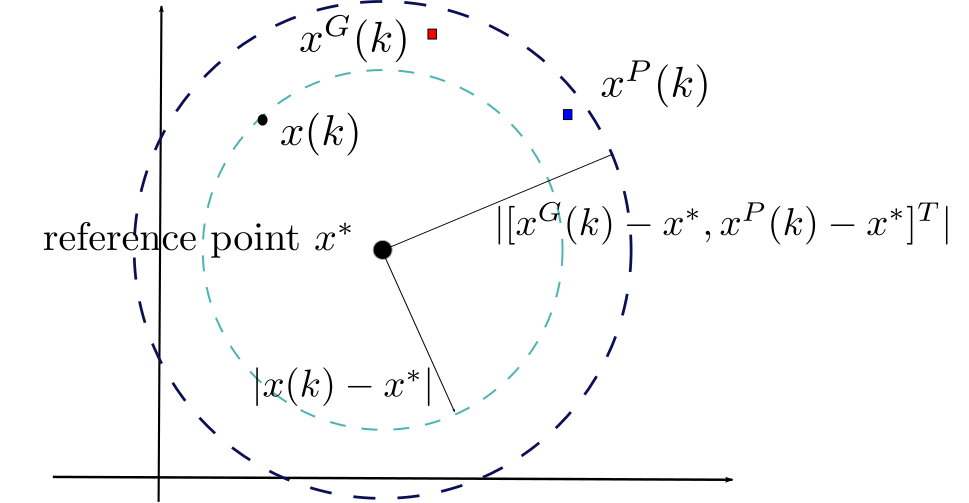
\includegraphics[width=0.6\linewidth]{./fig/boundary}
\caption{A bound on a particle's position by a reference point $ x^{*} $ from Equation \ref{eq:state_bound:conv}.
The ratio of wo radii indicates $ \gamma $.}
\label{fig:boundary}
\end{figure}

\begin{mycoro}
\label{coro:param_unit_disc}
Write $ A(k) = 
\begin{bmatrix}
\chi & - \chi \phi \\
\chi & 1 - \chi \phi
\end{bmatrix}
$, in which
$ \phi \in [0,  \phi^{P} + \phi^{G} ] $ and $ \chi \in ( 0, 1 ) $.
When $ \phi \in (0 , \frac{2(1+\chi)}{\chi} ) $, the system \eqref{eq:pso_up_linalg_simp} is input-to-state stable.
\begin{proof}
Let $ a = (1 + \chi) - \chi \phi $. 
The eigenvalues of $ A(k) $ are
$ \lambda = \frac{ a \pm \sqrt{ a^{2} - 4 \chi } }{2} $.

\begin{enumerate}
\item If $ a^{2} \geq 4 \chi $, we have $ a \geq 2 \sqrt{\chi} $ or $ a \leq - 2 \sqrt{\chi} $.

If $ a \geq 2 \sqrt{\chi} $, then $ | \lambda_{\max} | < 1 $ derives $ 0 < \frac{a-\sqrt{a^{2}-4\chi}}{2} \leq \frac{a+\sqrt{a^{2}-4\chi}}{2} < 1 $.
It means that $ 2 \sqrt{ \chi } \leq a < 1 + \chi $.

If $ a \leq 2 \sqrt{\chi} $, then $ | \lambda_{\max} | < 1 $ derives $ -1 < \frac{a-\sqrt{a^{2}-4\chi}}{2} \leq \frac{a+\sqrt{a^{2}-4\chi}}{2} < 0 $.
It means that $ - (\chi+1) < a \leq - 2 \sqrt{\chi} $.

\item If $ a^{2} \geq 4 \chi $, we have $ - 2 \sqrt{\chi} < a < 2 \sqrt{\chi} $.

$ | \lambda_{\max} | < 1 $ derives $ \frac{ a^{2} }{4} + \frac{ a^{2} - 4\chi }{4} < 1 $.
It means that $ - 2 \sqrt{ 2(1+\chi) } < a < 2 \sqrt{ 2(1+\chi) } $.
Because $ \sqrt{ 2(1+\chi) } > 2 \sqrt{ \chi } $, we have $ - 2 \sqrt{\chi} < a < 2 \sqrt{\chi} $.
\end{enumerate}
Combining these two cases, we have  $ - (1 + \chi) < a < 1 + \chi $.
It equals to $ \phi \in (0 , \frac{2(1+\chi)}{\chi} ) $.

\end{proof}
\end{mycoro}

Figure \ref{fig:paramSpace} shows the parameter space.
The x-axis is $ \phi = \phi^{P} + \phi^{G} $ and the y-axis is $ \chi $.
The stable region in red is obtained from eigenvalue test on Theorem \ref{thm:iss} and the yellow boundary is obtained from Corollary \ref{coro:param_unit_disc}.
\begin{figure}
\centering
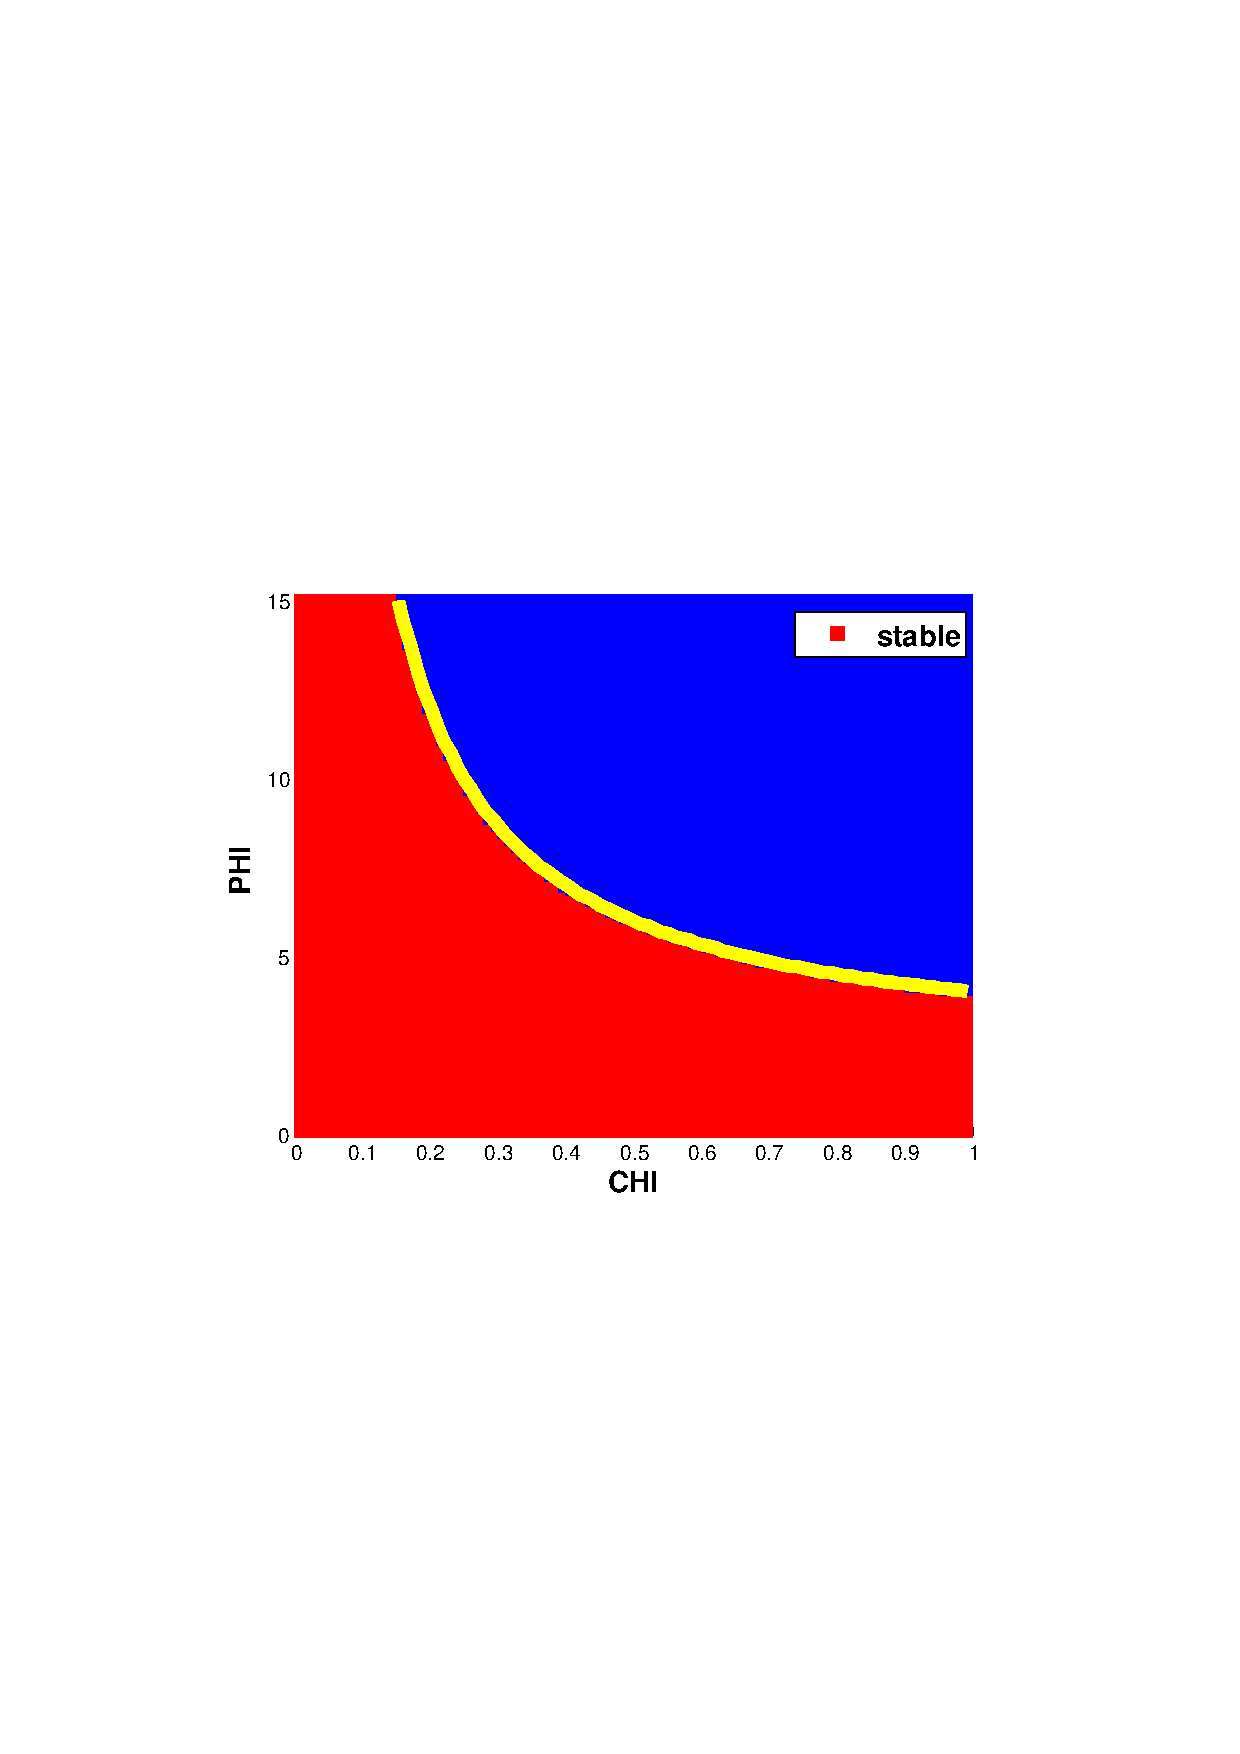
\includegraphics[width=0.5\linewidth]{./fig/param2}
\caption{Parameter space}
\label{fig:paramSpace}
\end{figure}


%Since by Theorem \ref{thm:iss} PSO is ISS, and therefore by Corollary \ref{coro:state_bound} the stability of the cascade system depends on the output of the input update component. We can say:
%\begin{enumerate}
%\item If the input update component generates converging personal best and global best, the bound of the particle position will converge;
%\item If the personal best and global best vary within a bound, the particle will converge within a bound;
%\item If the personal best and global best become constant, the particle will converge to a point.
%\end{enumerate}
%Furthermore, by equation \eqref{eq:state_bound}, we know that the convergence of a particle's position $ x(k) $ to $ x^{*} $ depends on how $ x^{P}(k) $ and $ x^{G}(k) $ converge to $ x^{*} $, if the position update component is input-to-state stable.
%In particular, the boundary of the distance between a particle's position and  $ x^{*} $ is determined by the initial distance $ x(0) -  x^{*} $, $ x^{P}(k) -  x^{*} $ and $ x^{G}(k) -  x^{*} $.

%Answer two questions here
% a) why we need iss of position update 
% b) what else do we need for iss

The input-to-state stability of the position update component makes the movement of a particle bounded in a range that covers the global best and the personal best.
This property provides the chance that the particle exploits the regions near around the personal best and the global best.
We can have:
\begin{enumerate}
\item If the personal best and global best converge, the bound of the particle position will converge;
\item If the personal best and global best vary within a bound, the particle will converge within a bound;
\item If the personal best and global best become constant, the particle will converge to a point.
\end{enumerate}
Furthermore, by \eqref{eq:state_bound}, we know that the convergence of a particle's position $ x(k) $ to $ x^{R} $ depends on how $ x^{P}(k) $ and $ x^{G}(k) $ converge to $ x^{R} $, if the position update component is input-to-state stable.
In particular, the boundary of the distance between a particle's position and  $ x^{R} $ is determined by the initial distance $ x(0) -  x^{R} $, $ x^{P}(k) -  x^{R} $ and $ x^{G}(k) -  x^{R} $.
Conversely, if the position update component is not input-to-state stable, the movement of the particle will diverge from the global best and the personal best.
The design of the exploitation by the personal best and the global best is lost.
%As in Figure \ref{fig:sys_flow}, the position update component and the input update component are serially connected.
When the position update component is input-to-state stable, the input-to-state stability of the particle is determined by the input-to-state stability of the personal best update component.
However, the input-to-state stability of the input update component depends on the fitness distribution, which could not be guaranteed in many cases.
In section \ref{sec:particle}, we will analyze the behavior of the particle when the position update component is input-to-state stable.
We will later extend the analysis to the swarm in section \ref{sec:swarm}.





\section{Particle analysis}
\label{sec:particle}


As in Figure \ref{fig:categorize_regions}, the solution space will be divided into three types of regions by the global best and the personal best.
\begin{itemize}
\item $ f(x) > f(x^G) $
Once a particle gets into this region, it updates both global best and personal best. 
It becomes a leader of the swarm.
\item $ f(x^{G}) > f(x) > f(x^{P}) $
Once a particle gets into this region, it updates only the personal best.
The solution space is then re-divided.
\item $ f(x) < f(x^{P}) $
When a particle is in this region, it only moves as a random walk.
\end{itemize}

\begin{figure}
\centering
\includegraphics[width=0.7\linewidth]{./fig/categorize_regions}
\caption{How global best and personal best divide the solution space.}
\label{fig:categorize_regions}
\end{figure}

The result of the movement of a particle is determined by which region of the solution space it moves in.

\subsection{One hill case}



\subsection{More than one hill case}



\section{Swarm analysis}
\label{sec:swarm}

\subsection{Consensus of a swarm}

Combinations of ISS parts are ISS

Swarm as such a combination

Conditions where update is ISS

trivially at stagnation
But also when on a single hill

Bound on swarm for the single hill case (perhaps as function of the width of the hill?
Or width of the hill as a percentage of the feasible region?)
test on 2-d case to show that the bound can prevent a particle    from reaching another hill.
This is one form of the swarm failing to converge the global optimal.

Can we look at parameters for the whole swarm?

\subsection{Value of a swarm}

Being on one hill is the unlikely case bound in the multi hill case.
Might not seem useful but is the essence of what makes a swarm a swarm.
Bounds the swarm to a region around p-bests where g-best has been unable to pull other particles to its hill.
For a function with narrow hills, g-bests on a narrow hills is less likely to capture another particle, thus the swarm searches more, for functions with broad hills, p-gest are more likely to be pulled to g-bests hill and search there.
Thus swarm diversity is the mechanism that allows the swarm to not converge when searching is likely needed but focus and converge when the fitness landscape appear to favor exploitation.
This does not happen at stagnation and does not happen without multiple members. <need to say this in a more mathematical way>>

example ?? function for exploration case
example sphere function for the exploitation case
try to use bound as a function of hill width metric

Rastrigin as a counter example? Does it get stuck or just sample for ever? It certainly runs longer.

\subsection{Diversity injection}

Work with the Rastrigin function has lead others to experiment with diversity injection to prevent pre-mature convergence (or prevent convergence at all)
I am not sure, do we want it to converge? ever?
On what basis would I propose a new algorithm?
Show that it would converge based on ISS?

\section{Conclusion}

\begin{frame}{Conclusion}{$ \null $}

\begin{itemize}
\item decomposed-based multi-objective optimization
\item efficient way of finding the Pareto optimal paths
%\item 
\end{itemize}

\end{frame}

\begin{frame}{$ \null $}{$ \null $}

\centering
\Huge Thank you

\end{frame}

\bibliographystyle{IEEEtran}
\bibliography{reference}

\appendix

\begin{frame}

\begin{minipage}{\textwidth}
\begin{center}
Thank you!
\end{center}
\end{minipage}


\end{frame}

\end{document}

